%/*
% * SPDX-FileCopyrightText: 2021 Stefan Begerad <stefan@begerad.de>
% *
% * SPDX-License-Identifier: GPL-3.0-or-later
% */

%make document a Beamer presentaion
\documentclass{beamer}

%include preamble
%/*
% * SPDX-FileCopyrightText: 2021 Stefan Begerad <stefan@begerad.de>
% *
% * SPDX-License-Identifier: GPL-3.0-or-later
% */

%define outer theme (color and background)
%\usetheme{default}
%\usetheme{Goettingen}
%\usetheme{Darmstadt}
%\usetheme{Copenhagen}
\usetheme{Boadilla}
%\usetheme{Berlin}
%\usetheme{Berkeley}
%\usetheme{Bergen}
%\usetheme{Antibes}
%\usetheme{AnnArbor}
%\usetheme{Warsaw}
%\usetheme{Szeged}

%define color of theme
%\usecolortheme{default}
%\usecolortheme{beaver}
\usecolortheme{seahorse}

%add the following package to use links
%Define hyperref as last package, because it modifies other instructions!
\usepackage{hyperref}

\title[Dede]%optional
{Dede Echtzeit-Karte}

\subtitle{Offen, Unabhängig, Universell}

\author[Begerad]%(optional, for multiple authors)
{Stefan~Begerad}

\date[OTM, 6.2.2021]%(optional)
{Open Transport Meetup, June 2. 2021}

\logo{
\includegraphics[height=1cm]{dede/dedeLogo0128}}


%define the document
\begin{document}

%define title page
\begin{frame}
  \titlepage
\end{frame}

%outline table of content for the entire presentation
%use asterisk to indicate that this section shall not be part of the table
%the name of the section serves as the title of the slide
\AtBeginSection[]
{
    \begin{frame}
        \frametitle{Inhalt}
        \tableofcontents[currentsection]
    \end{frame}
}

\section{Dede Echtzeit-Karte}

%/*
% * SPDX-FileCopyrightText: 2021 Stefan Begerad <stefan@begerad.de>
% *
% * SPDX-License-Identifier: GPL-3.0-or-later
% */

\bgroup

\usebackgroundtemplate{%
\tikz\node[opacity=1,inner sep=0] {
   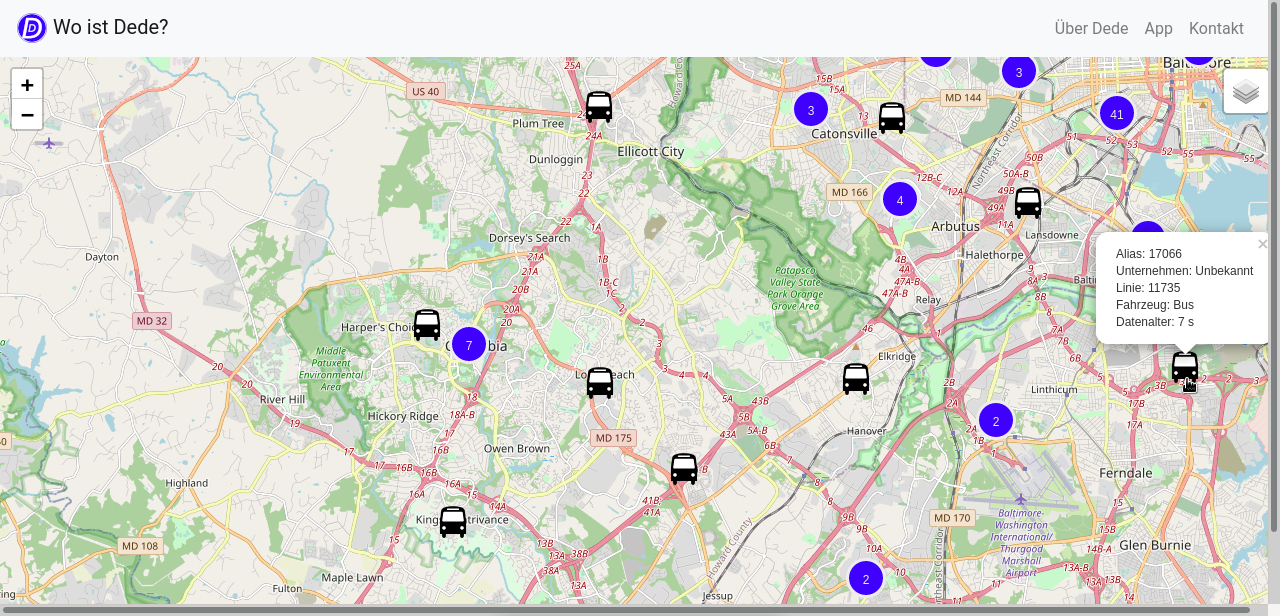
\includegraphics[width=\paperwidth]{dede/dede_real-time_map_crop}};
}

\begin{frame}{Dede Echtzeit-Karte}
\end{frame}

\egroup



\bgroup

\usebackgroundtemplate{%
\tikz\node[opacity=0.15,inner sep=0] {
   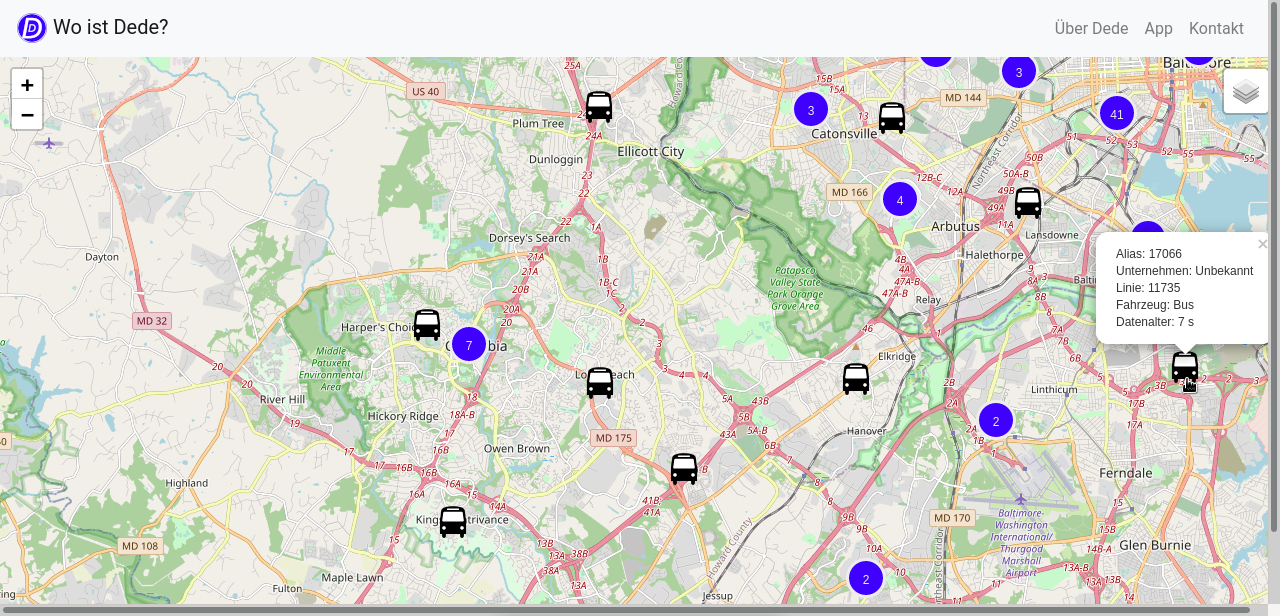
\includegraphics[width=\paperwidth]{dede/dede_real-time_map_crop}};
}

%/*
% * SPDX-FileCopyrightText: 2021 Stefan Begerad <stefan@begerad.de>
% *
% * SPDX-License-Identifier: GPL-3.0-or-later
% */

\begin{frame}{Dede Philosophie}
  Dede: eine freie, unabhängige und universelle Echtzeit-Karte
  \begin{itemize}
  \item FREI: Gemeinschaftsprojejt als freie Software (wie in Redefreiheit und NICHT wie in Freibier;-)) veröffenlicht\footnote{\url{https://github.com/dancesWithCycles/dede-front-end}}
  \item UNABHÄNGIG: weder ausgerüstete Fahrzeugflotte noch eigene IT-Infrastuktur notwendig
  \item UNIVERSELL: beliebige Fahrzeuge wie Bahn, Bus, Car-Sharing, Fahrdienst, Straßenbahn, Tram, Taxi, usw. universell darstellt
  \end{itemize}
\end{frame}


%/*
% * SPDX-FileCopyrightText: 2021 Stefan Begerad <stefan@begerad.de>
% *
% * SPDX-License-Identifier: GPL-3.0-or-later
% */

\begin{frame}{Dede Konzept}
  Das System Dede Echtzeit-Karte besteht aus \textbf{drei} Komponenten:\\
  \begin{itemize}
  \item Dede Bordrechner,
  \item Dede Server und
  \item Dede Karte.
  \end{itemize}
  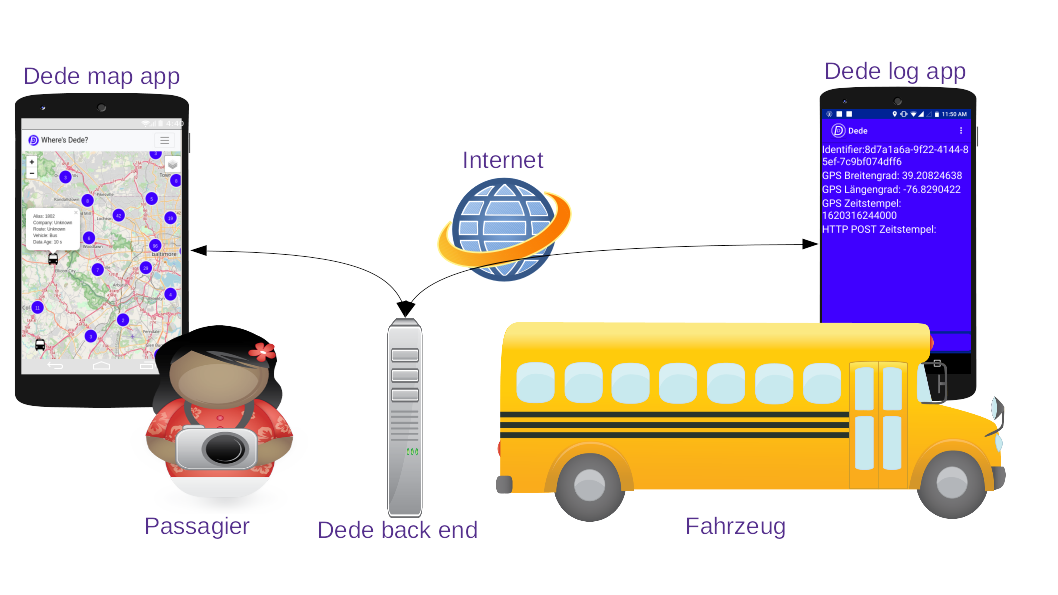
\includegraphics[width=0.8\paperwidth]{dede/dede-concept}
\end{frame}


%/*
% * SPDX-FileCopyrightText: 2021 Stefan Begerad <stefan@begerad.de>
% *
% * SPDX-License-Identifier: GPL-3.0-or-later
% */

\begin{frame}{Dede Bordrechner}
  Der \textbf{Dede Boardrechner} für Smartphones zeichnet die Bewegungsdaten des Fahrzeugs auf und überträgt sie per Internet an den \textbf{Dede Server}.
  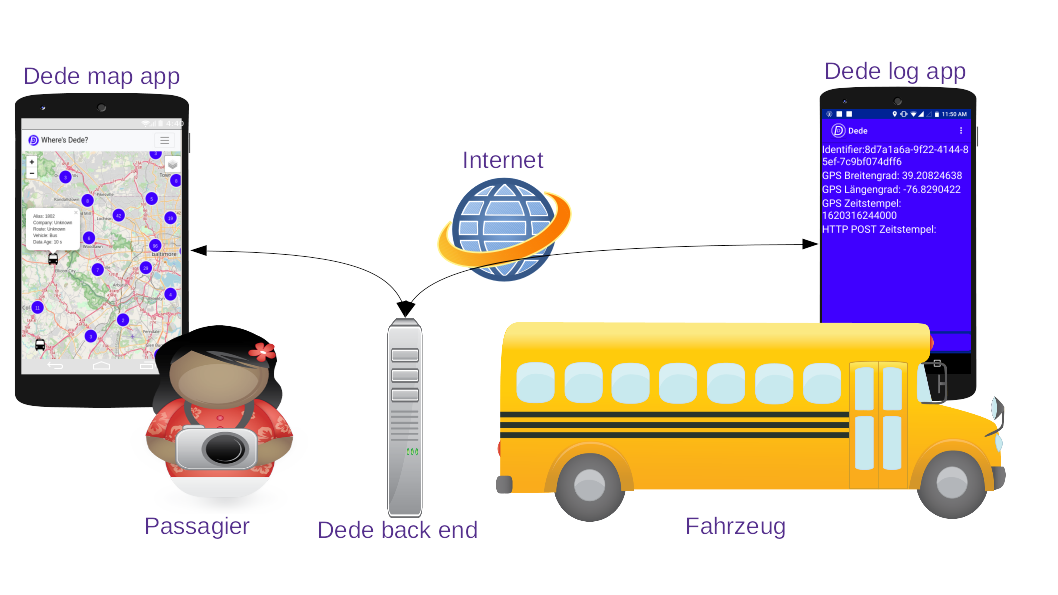
\includegraphics[width=\paperwidth]{dede/dede-concept}
\end{frame}

\begin{frame}{Dede Bordrechner im Detail}
  \begin{itemize}
  \item App für Android Smartphone
  \item Investitionskosten pro Fahrzeug: gängiges Android Smartphone für die Installation der kostenlosen App genügt
  \item Betriebskosten pro Farhzeug: keine
    \begin{itemize}
    \item Lizenskosten: keine
    \item Supportkosten: keine
    \end{itemize}
  \item Interaktion mit
    \begin{itemize}
    \item \textbf{Dede Server} per Digitalfunk (SIM-Karte für Mobilfunk)
    \item Ortung per GPS
    \end{itemize}
  \end{itemize}
  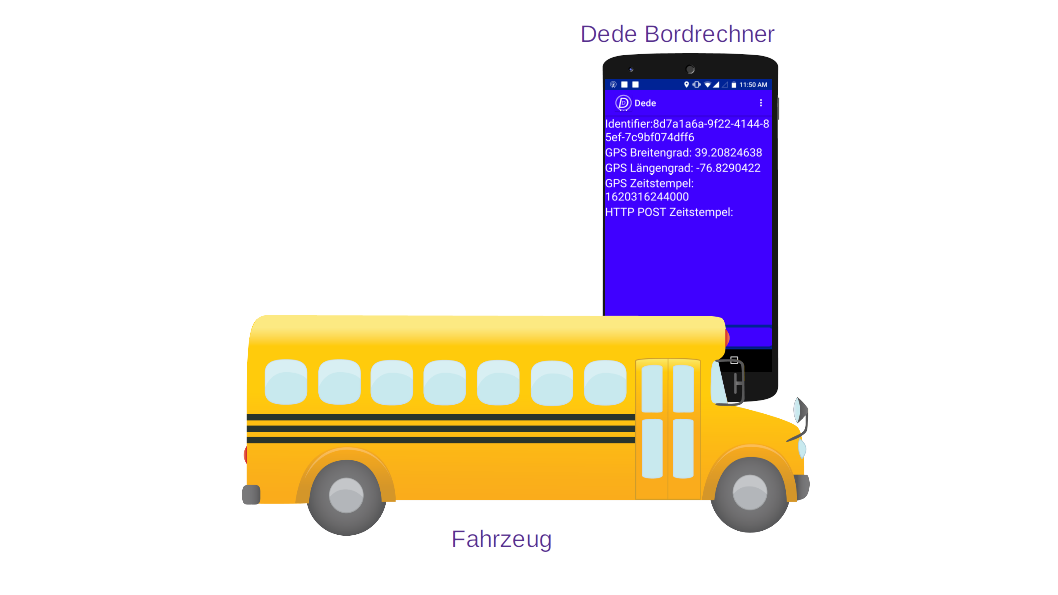
\includegraphics[width=0.5\textwidth]{dede/dede-on-board-computer-june-04.png}
\end{frame}

\begin{frame}{Dede Bordrechner im Detail}
  \center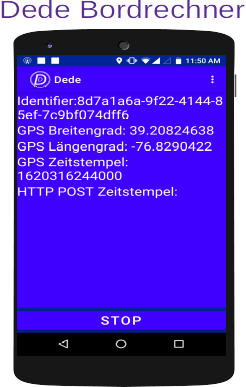
\includegraphics[width=0.4\textwidth]{dede/dede-on-board-computer-only-june-04.png}
\end{frame}


%/*
% * SPDX-FileCopyrightText: 2021 Stefan Begerad <stefan@begerad.de>
% *
% * SPDX-License-Identifier: GPL-3.0-or-later
% */

\begin{frame}{Konventioneller Bordrechner}
  \begin{itemize}
  \item Im Fahrzeug fest verbaut und mit Strom- und Datennetz verbunden
  \item Investitionskosten pro Fahrzeug: etwa 2 bis 3 Tausend Euro
  \item Betriebskosten pro Farhzeug: im Bereich von 1 bis 5 Prozent p.a.
    \begin{itemize}
    \item Lizenskosten
    \item Supportkosten
    \end{itemize}
  \item Interaktion mit
    \begin{itemize}
    \item Fahrzeugnetz bspw. IBIS,
    \item Ticket-Drucker oder -Scanner,
    \item Anzeige für Fahrdienst,
    \item Leitstelle per Analog- oder Digitalfunk (SIM-Karte für Mobilfunk)
    \item Ortung per GPS
    \end{itemize}
  \end{itemize}
  
\includegraphics[width=0.5\textwidth]{public-transport/bus.png}
\end{frame}



%/*
% * SPDX-FileCopyrightText: 2021 Stefan Begerad <stefan@begerad.de>
% *
% * SPDX-License-Identifier: GPL-3.0-or-later
% */

\begin{frame}{Dede Server}
  Der \textbf{Dede Server} vermittelt zwischen \textbf{Dede Boardrechner} und \textbf{Dede Karte}, so das die Karte \textbf{NICHT} jeden Boardrechner separat abfragen muss.
  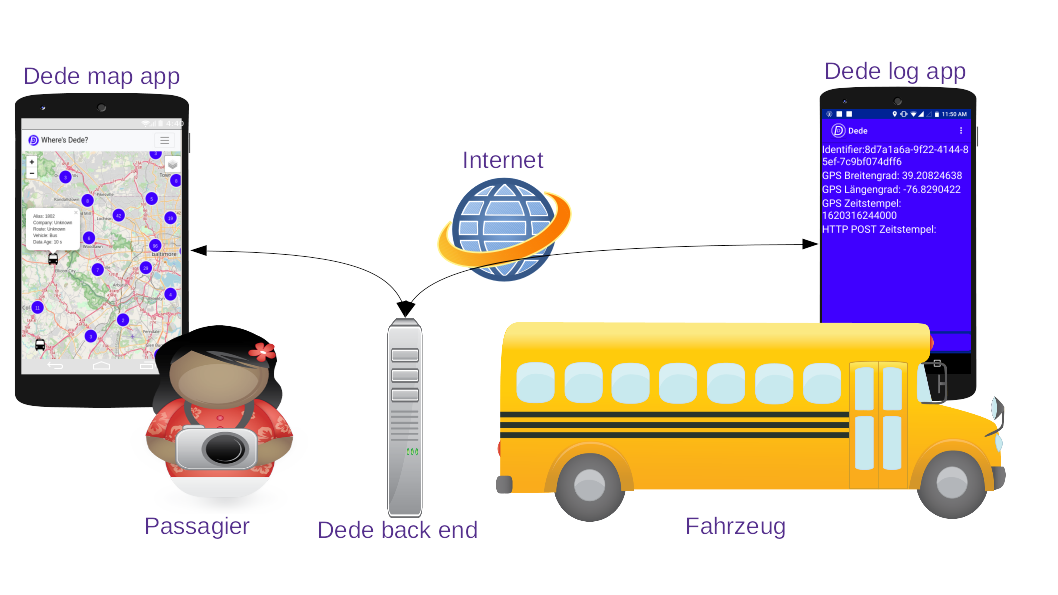
\includegraphics[width=\paperwidth]{dede/dede-concept}
\end{frame}


%/*
% * SPDX-FileCopyrightText: 2021 Stefan Begerad <stefan@begerad.de>
% *
% * SPDX-License-Identifier: GPL-3.0-or-later
% */

\begin{frame}[fragile]
\frametitle{Dede Server: Datenbankmodel}
\begin{lstlisting}
const vehicleSchema=new Schema({
    uuid:{type:String,required:true,unique:true},
    lat:{type:Number,min:-90,max:90},
    lon:{type:Number,min:-180,max:180},
    ts:{type:Number,min:0},
    alias:String,
    vehicle:String,
    label:String,
    licensePlate:String,
    tripId:String,
    routeId:String,
    directionId:String,
    startTime:String,
    startDame:String
})
\end{lstlisting}
\end{frame}

%\begin{frame}{Dede Server: Datenbankmodel}[fragile]
%  \begin{lstlisting}
%  \begin{lstlisting}[caption=Datenbankmodel]
%  \end{lstlisting}
%\end{frame}


%/*
% * SPDX-FileCopyrightText: 2021 Stefan Begerad <stefan@begerad.de>
% *
% * SPDX-License-Identifier: GPL-3.0-or-later
% */

\begin{frame}{Dede Karte}
  Die \textbf{Dede Karte} visualisiert die Bewegungdaten auf einer Karte in Echtzeit.
  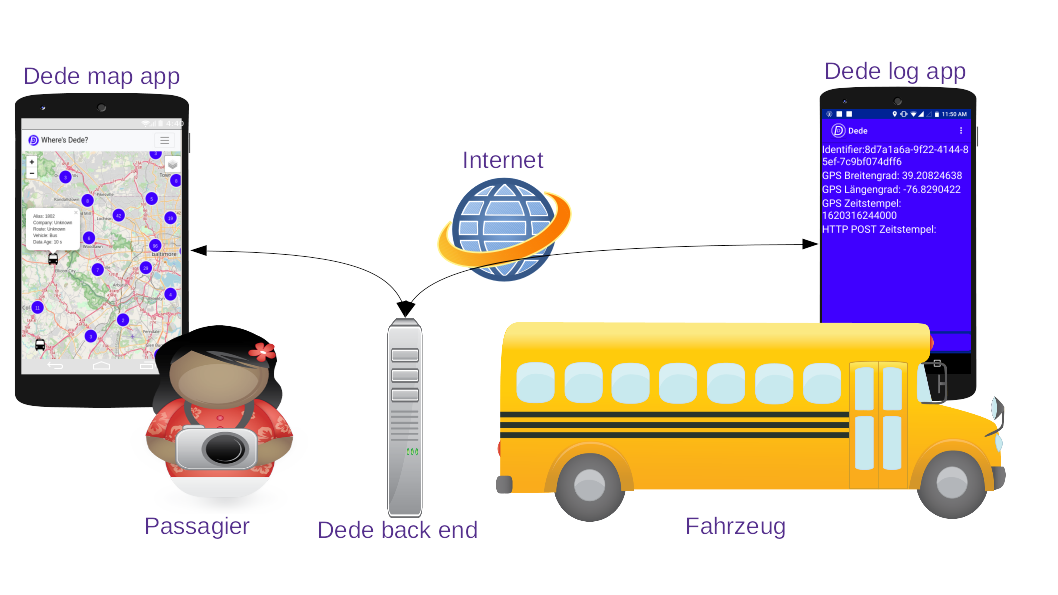
\includegraphics[width=\paperwidth]{dede/dede-concept}
\end{frame}

\bgroup

\usebackgroundtemplate{%
\tikz\node[opacity=1,inner sep=0] {
   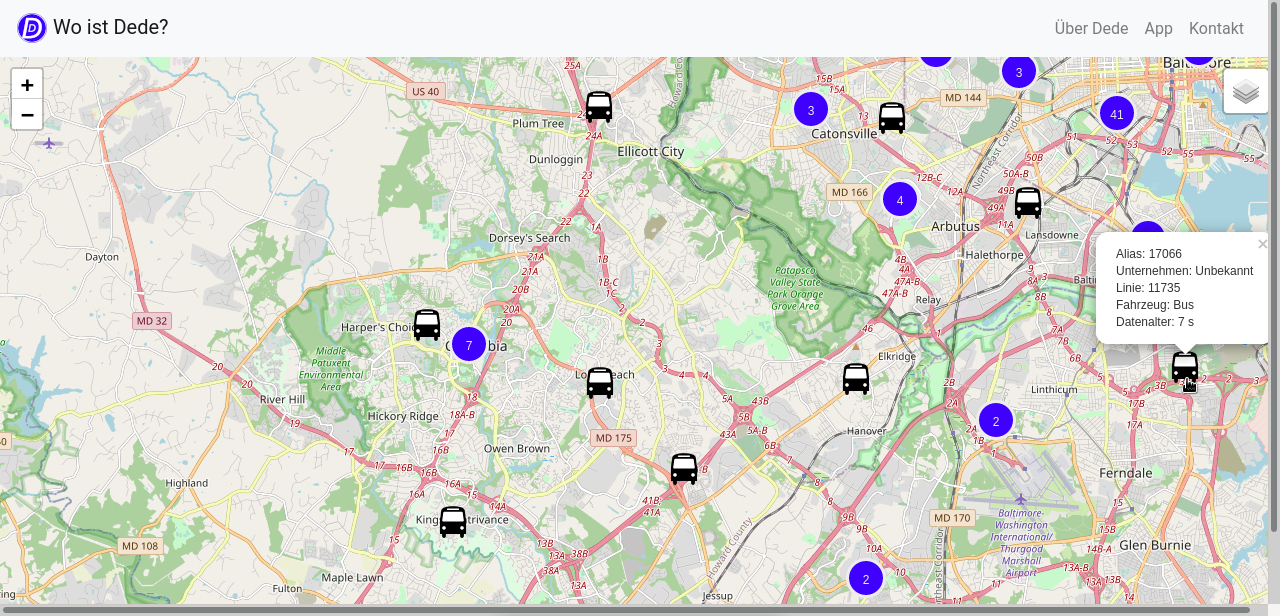
\includegraphics[width=\paperwidth]{dede/dede_real-time_map_crop}};
}

\begin{frame}{Dede Karte}
\end{frame}

\egroup


%/*
% * SPDX-FileCopyrightText: 2021 Stefan Begerad <stefan@begerad.de>
% *
% * SPDX-License-Identifier: GPL-3.0-or-later
% */

\begin{frame}{Dede Integration}
  \begin{itemize}
  \item Betrieblich:
    \begin{itemize}
    \item Ein Fahrzeug erscheint in Echtzeit auf der \textbf{Dede Karte}, sobald der Fahrdienst die App \textbf{Dede Bordrechner} aktiviert.
    \item Ein Fahrzeug wird von der \textbf{Dede Karte} in Echtzeit entfernt, sobald der Fahrdienst die App \textbf{Dede Bordrechner} deaktiviert.
      \item In der App \textbf{Dede Bordrechner} kann der Fahrdienst Details zu Betreiber, Nummer und Richtung bei Bedarf eingestellen.
    \end{itemize}
  \item Technisch:
    \begin{itemize}
    \item Pro Fahrzeug ist vom Fahrdienst ein Smartphone mit Android Betriebssystem mitzuführen.
    \item Das Smartphone muss jederzeit aktiv sein mit einer ständigen Stromversorgung und Internet-Verbindung (bspw. per Mobilfunk).
    \end{itemize}
  \end{itemize}
\end{frame}


%/*
% * SPDX-FileCopyrightText: 2021 Stefan Begerad <stefan@begerad.de>
% *
% * SPDX-License-Identifier: GPL-3.0-or-later
% */

\begin{frame}
  \frametitle{Datenaufkommen über Mobilfunk}
  Dede Bordrechner und Dede Server tauschen Daten per Mobilfunk aus.
  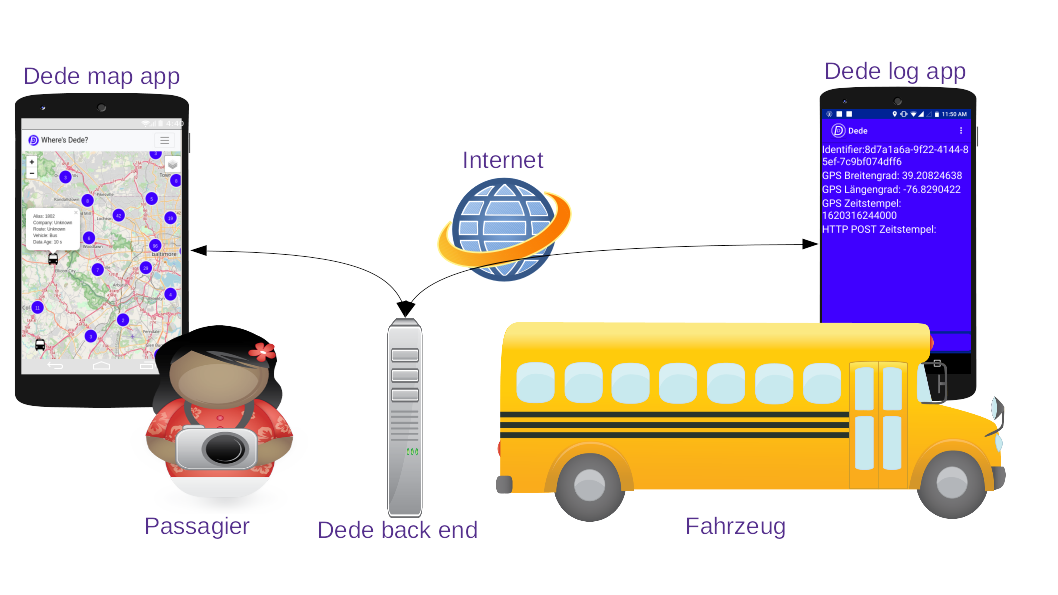
\includegraphics[width=\paperwidth]{dede/dede-concept}
\end{frame}

\begin{frame}
  \frametitle{Datenaufkommen über Mobilfunk}
  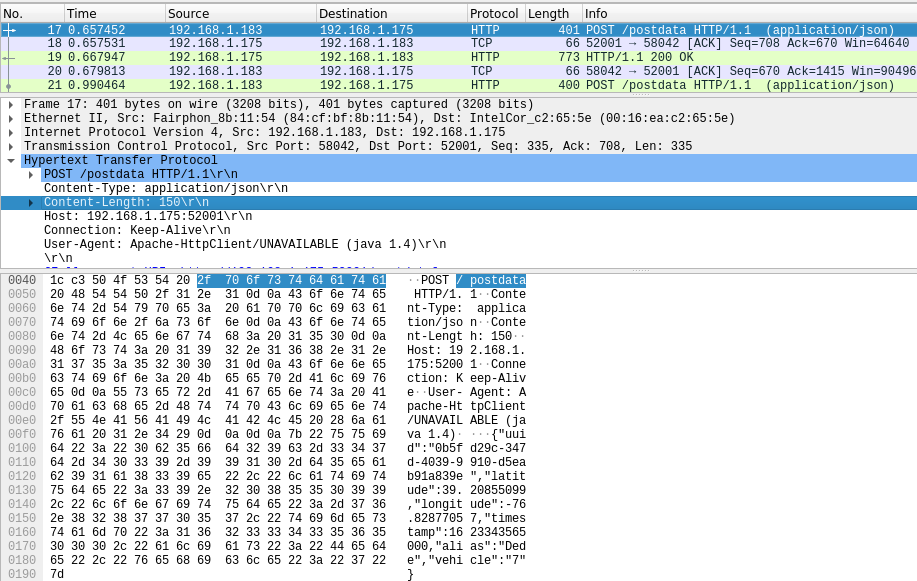
\includegraphics[width=0.88\paperwidth]{dede/dede-obc-wireshark-http-post}
\end{frame}

\begin{frame}
  \frametitle{Datenaufkommen über Mobilfunk}
  \begin{itemize}
  \item Pro Positionserfassung erstellt der Dede Bordrechner ein Datenobjekt in einer Größe von 150 Byte.
  \item Der Dede Bordrechner sendet eine HTTP POST-Anfrage in einer Größe von 401 Byte.
  \item Es resultiert ein Datenaufkommen von 1239 Byte pro Positionserfassung.
  \end{itemize}
  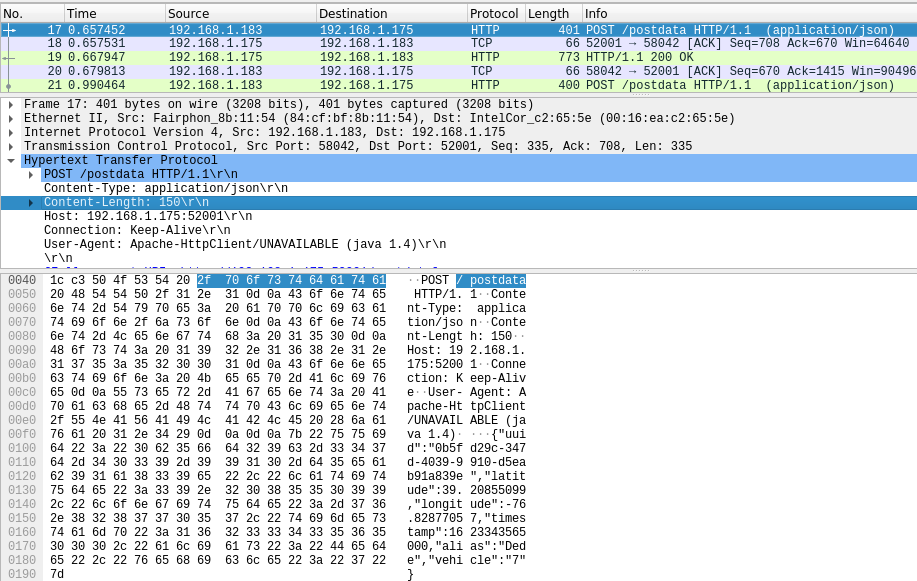
\includegraphics[width=0.5\paperwidth]{dede/dede-obc-wireshark-http-post}
\end{frame}

\begin{frame}
  \frametitle{Datenaufkommen über Mobilfunk}
  Annahme: Der Dede Bordrechner erfasst die Position einmal pro Minute.
  \begin{itemize}
  \item Datenaufkommen pro Minute: 1239 Byte/ 1,24 KByte
  \item Datenaufkommen pro Stunde: 74,34 KByte
  \item Datenaufkommen pro Tag: 1,78 MByte
  \item Datenaufkommen pro Monat: 55,31 MByte
  \item Datenaufkommen pro Jahr: 651,22 MByte
  \end{itemize}
  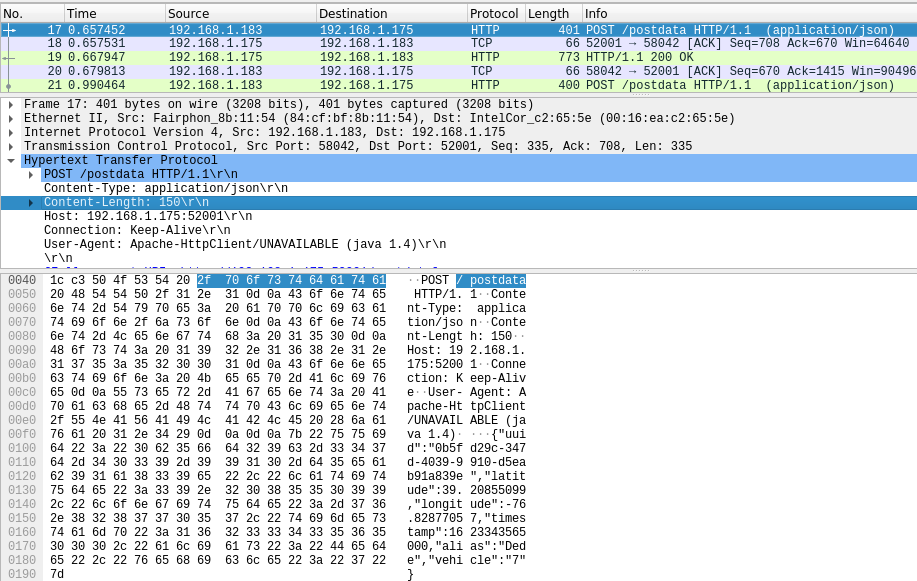
\includegraphics[width=0.5\paperwidth]{dede/dede-obc-wireshark-http-post}
\end{frame}


\begin{frame}{Danke!}
  \center {\huge\textbf{Dede Echtzeit-Karte www.dedriver.org}}
  \center {\Huge\textbf{Fragen?}}
\end{frame}

\egroup

\end{document}
